\documentclass[runningheads,a4paper]{llncs}

%
\usepackage{amssymb}
\usepackage{amsmath}
\usepackage{url}
\usepackage{graphicx}
\usepackage{multirow}
%
\newcommand{\argmin}[1]{\underset{#1}{\operatorname{arg}\operatorname{min}}\;}
\mathchardef\mhyphen="2D
\raggedbottom 
%
% Allow easy processing of labeled images in figures
\newcounter{lfigcounter}
\newenvironment{IonTab}{\begin{table}[htb]}{\end{table}}
\newenvironment{IonFig}{\setcounter{lfigcounter}{1}\begin{figure}} {\end{figure}}
\newenvironment{IonFigH}{\setcounter{lfigcounter}{1}\begin{figure}[h]}{\end{figure}}
\newenvironment{IonFigT}{\setcounter{lfigcounter}{1}\begin{figure}[!t]}{\end{figure}}
\newenvironment{IonFigB}{\setcounter{lfigcounter}{1}\begin{figure}[b]}{\end{figure}}
\def\ionbox#1{\makebox[#1]{(\alph{lfigcounter})}\stepcounter{lfigcounter}}
%
\begin{document}

\mainmatter  % start of an individual contribution

% first the title is needed
\title{An Image-based method for phase estimation, gating and temporal super-resolution of \\cardiac ultrasound}

% a short form should be given in case it is too long for the running head
\titlerunning{Image-based Phase Estimation Method for Cardiac Ultrasound}

% the name(s) of the author(s) follow(s) next
%
% NB: Chinese authors should write their first names(s) in front of
% their surnames. This ensures that the names appear correctly in
% the running heads and the author index.
%

% anonymous stuff
\author{*}
\authorrunning{*}   
\tocauthor{*}
\institute{*}

\maketitle

\begin{abstract}
Point-of-care low-cost hand-held ultrasound devices are emerging as an increasingly effective tool for rapid non-invasive visual assessment of cardiac structure and function on the bed-side. Their diagnostic value can be enriched further by coupling them with automated image analysis algorithms to accurately detect and quantify any cardiac abnormalities at the point-of-care potentially even in asymptomatic patients. However, a major challenge to this is the poor spatio-temporal resolution and high noise level of images obtained using these devices. In an effort to address this problem, we present a novel method for de-noising, gating, and temporal super-resolution of noisy low frame-rate periodic image sequences such as the ones obtained using low-cost hand-held cardiac ultrasound devices. 

We first transform the complex high-dimensional periodic cardiac ultrasound image sequence to a narrow-band 1D time series with the same periodicity characteristics using a novel strategy based on inter-frame similarity. Next, we decompose this time series use a trend extraction technique to obtain the trend/respiration and residual/heart-beat component signals. Next, we use the Hilbert transform to estimate the instantaneous cardiac and respiratory phases of each frame to facilitate gating and temporal super-resolution. Lastly, we use kernel regression with a novel kernel to learn an image manifold parametrized by instantaneous cardiac phase that can be sampled to generate a single-cycle video at a higher temporal-resolution. We demonstrate and validate our methods using cardiac ultrasound videos and associated ECG recordings of 6 mice.
%\keywords{Cardiac, Ultrasound, Phase estimation, Gating, Temporal super-resolution}
\end{abstract}

\vspace{-0.5cm}
\section{Introduction}
\label{sec:intro}
%

%

%\vspace{-0.5cm}
\section{Method}
\label{sec:method}
%
In this section, we present the theory underlying the proposed methods for instantaneous phase estimation, gating and temporal super-resolution of cardiac ultrasound videos. Specifically, we begin by describing our method for the estimation of instantaneous cardiac and respiratory phases in Section \ref{sec:method:phase_estimation}. We then present a robust method that uses these phase estimates to gate out video frames predominantly influenced by respiratory motion in Section \ref{sec:method:gating}. Finally, in Section \ref{sec:method:super_resolution}, we present a kernel regression method that uses the phase-tagged image sequence to reconstruct a single-period video at higher-temporal resolution. 
%
%
\begin{IonFigT}
\centering
%
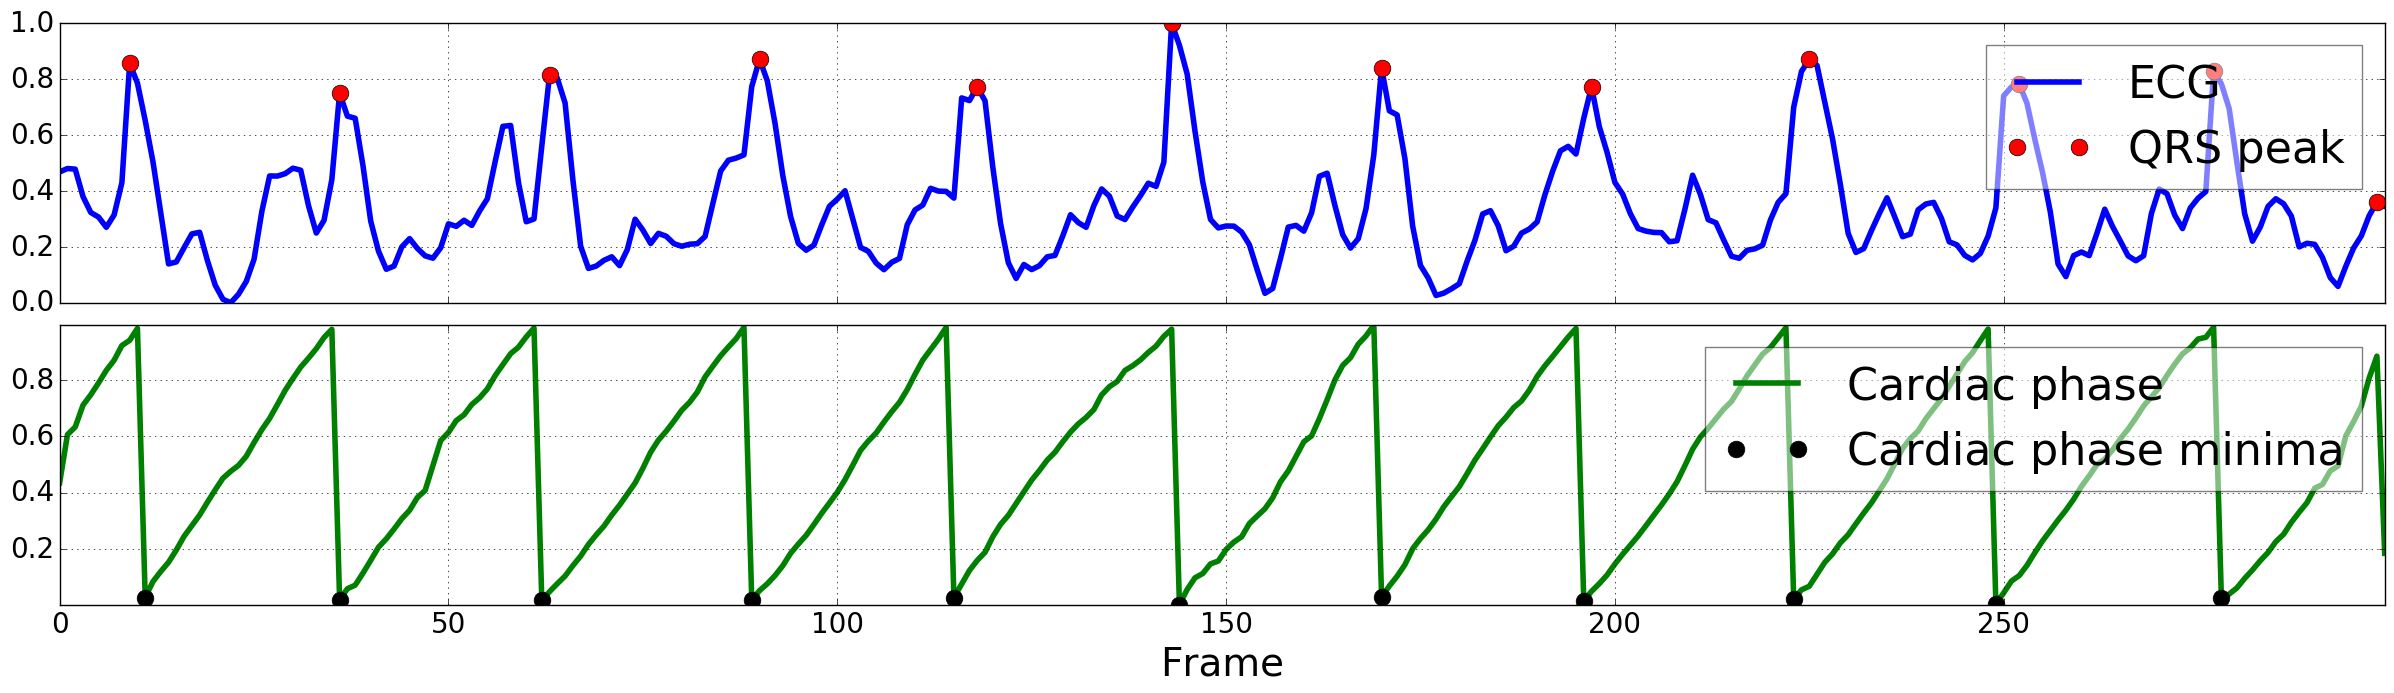
\includegraphics[width=5.0in]{figures/decoded/2015-07-27-10-36-06_2015-07-15-16-56-16_1.raw.bmode/ecg_instaphase_overlay.png}\\
\ionbox{5.0in}\\
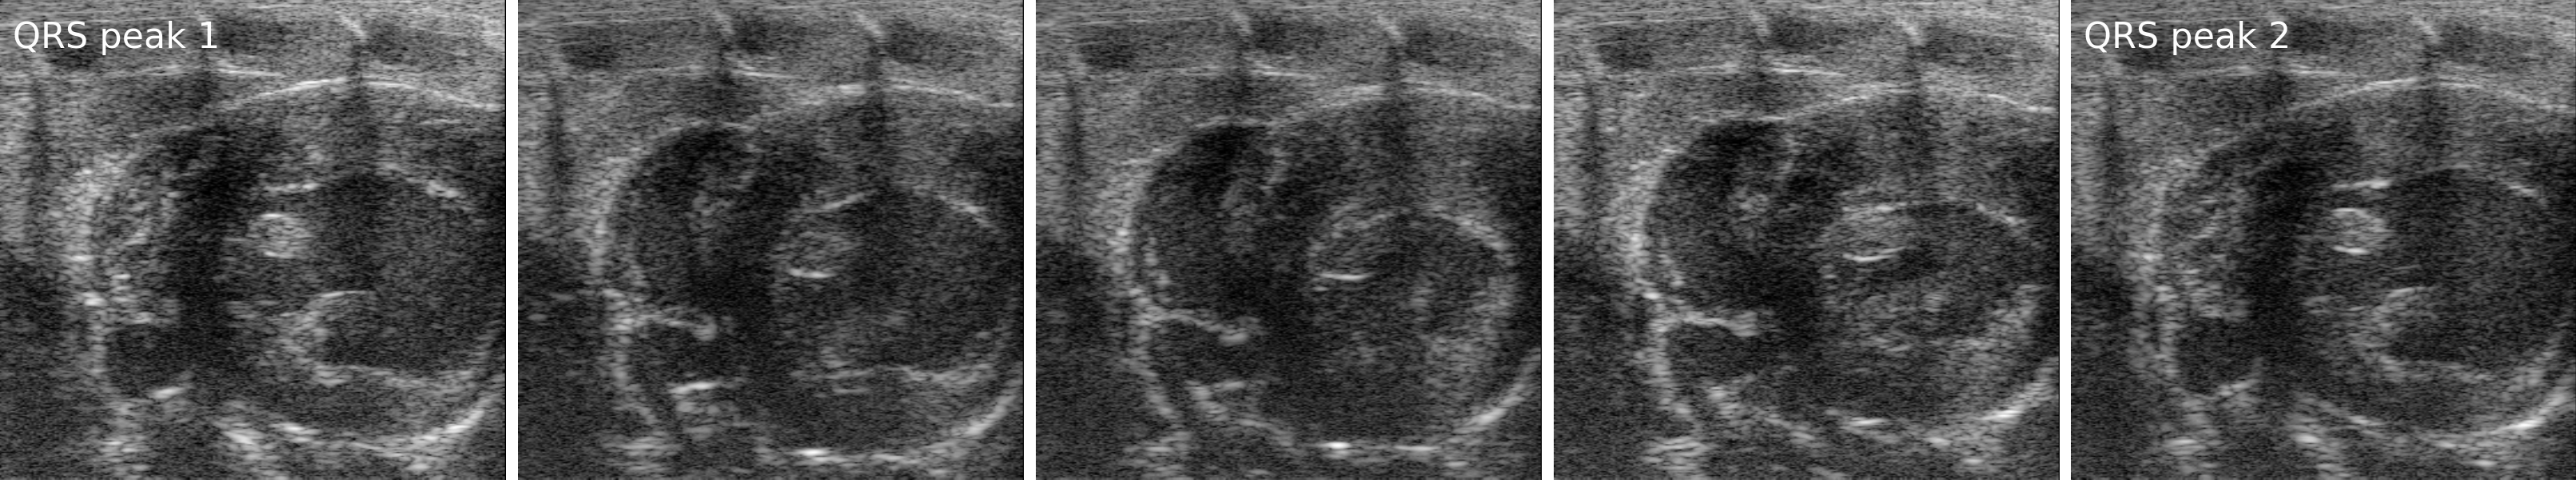
\includegraphics[width=5.0in]{figures/decoded/2015-07-27-10-36-06_2015-07-15-16-56-16_1.raw.bmode/qrs_peak_to_peak.png}
\ionbox{5.0in}\\
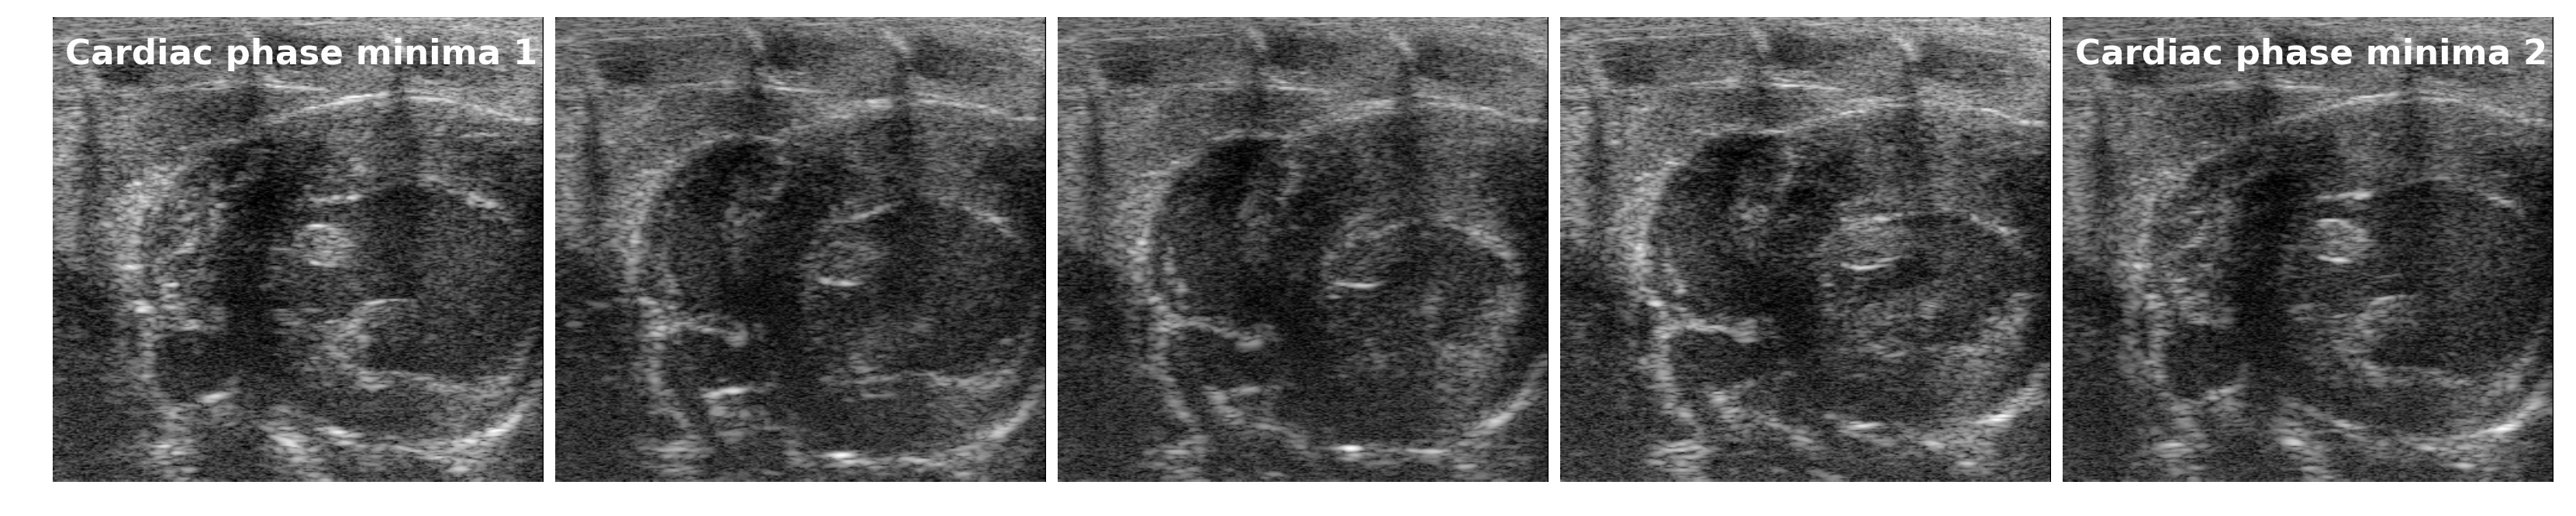
\includegraphics[width=5.0in]{figures/decoded/2015-07-27-10-36-06_2015-07-15-16-56-16_1.raw.bmode/instaphase_valley_to_valley.png}
\ionbox{5.0in}\\
%
\caption{Illustration of correspondence between ECG and the instantaneous cardiac phase estimated using the proposed method: (a) ECG signal (blue) and the cardiac phase estimated using our method using only image data. Also shown are the peaks of the QRS complex (pink circle) and the minima of the estimated cardiac phase (black circle) that correspond to the QRS peaks, (b) Five video frames evenly spaced in time between the first and second QRS peaks of the ECG signal constituting one cardiac cycle, and (c) Five video frames evenly spaced in time between first and second minima of the estimated cardiac phase constituting one cardiac cycle.}
\label{fig:instaphase_vs_ecg}
\end{IonFigT}
%\vspace{-0.5cm}
\subsection{Estimation of instantaneous cardiac and respiratory phases}
\label{sec:method:phase_estimation}
%
\begin{IonFigT}
\centering
%
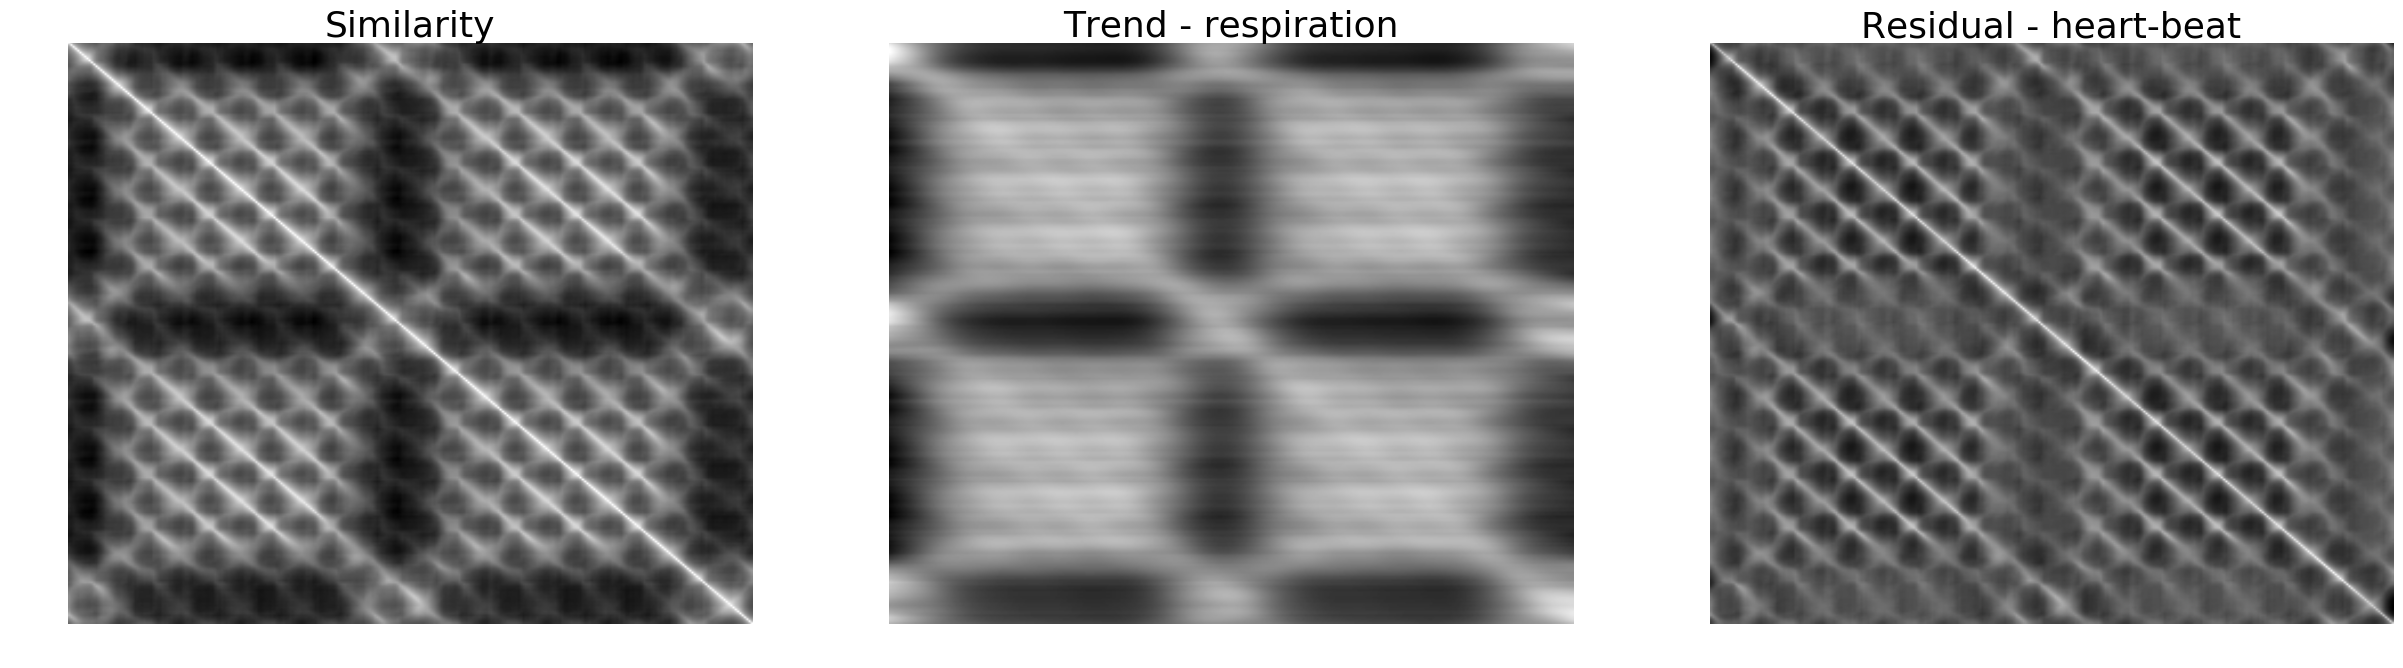
\includegraphics[width=4.75in]{figures/decoded/2015-07-27-10-36-06_2015-07-15-16-56-16_1.raw.bmode/simMat.png}
\ionbox{1.6in}\ionbox{1.6in}\ionbox{1.6in}\\
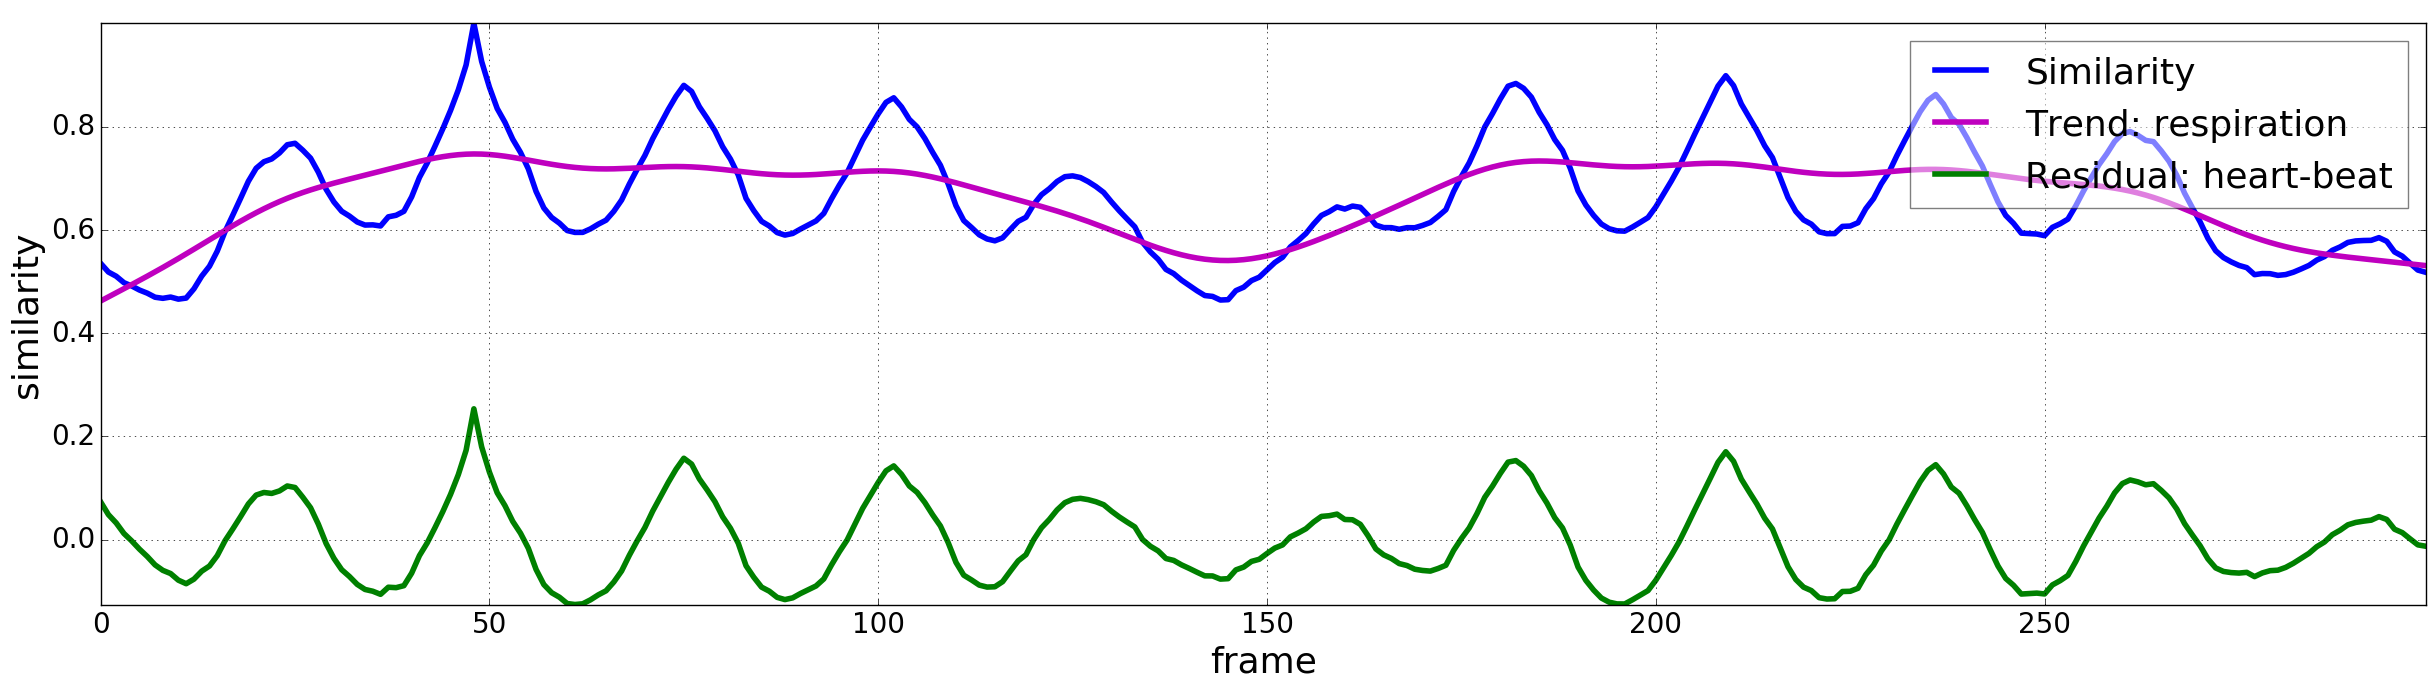
\includegraphics[width=4.75in]{figures/decoded/2015-07-27-10-36-06_2015-07-15-16-56-16_1.raw.bmode/season_trend_decomposition.png}
\ionbox{4.75in}\\
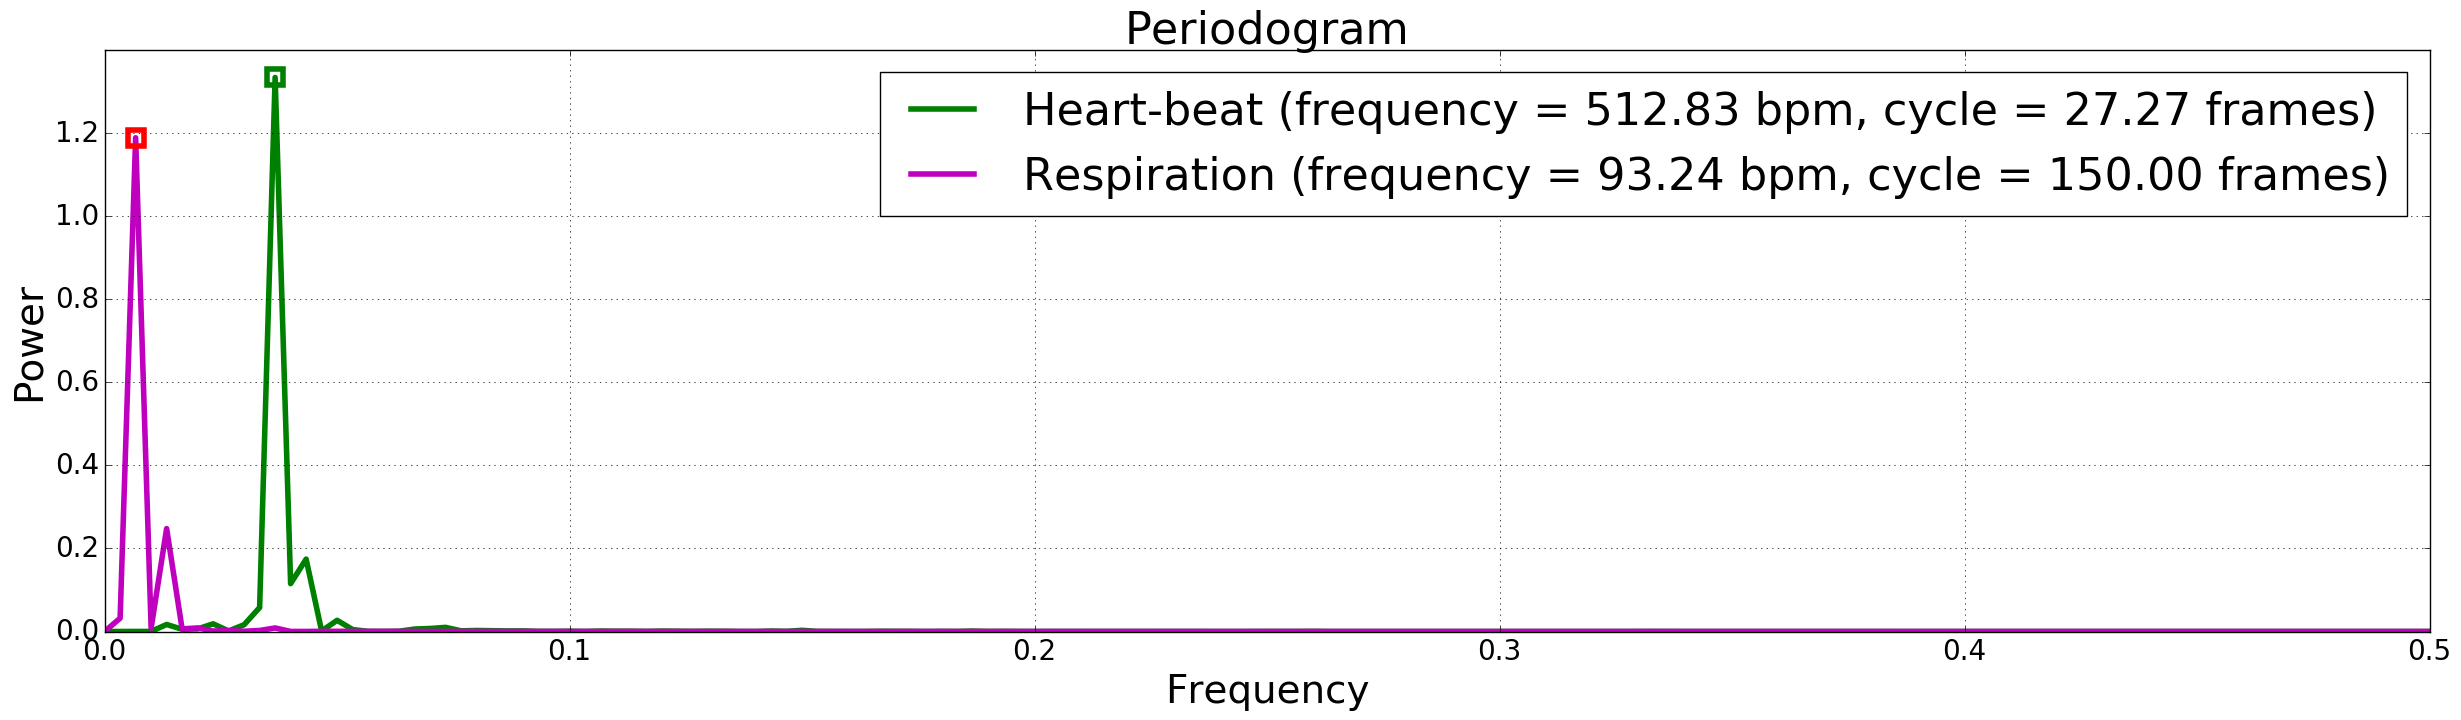
\includegraphics[width=4.75in]{figures/decoded/2015-07-27-10-36-06_2015-07-15-16-56-16_1.raw.bmode/periodogram.png}
\ionbox{4.75in}\\
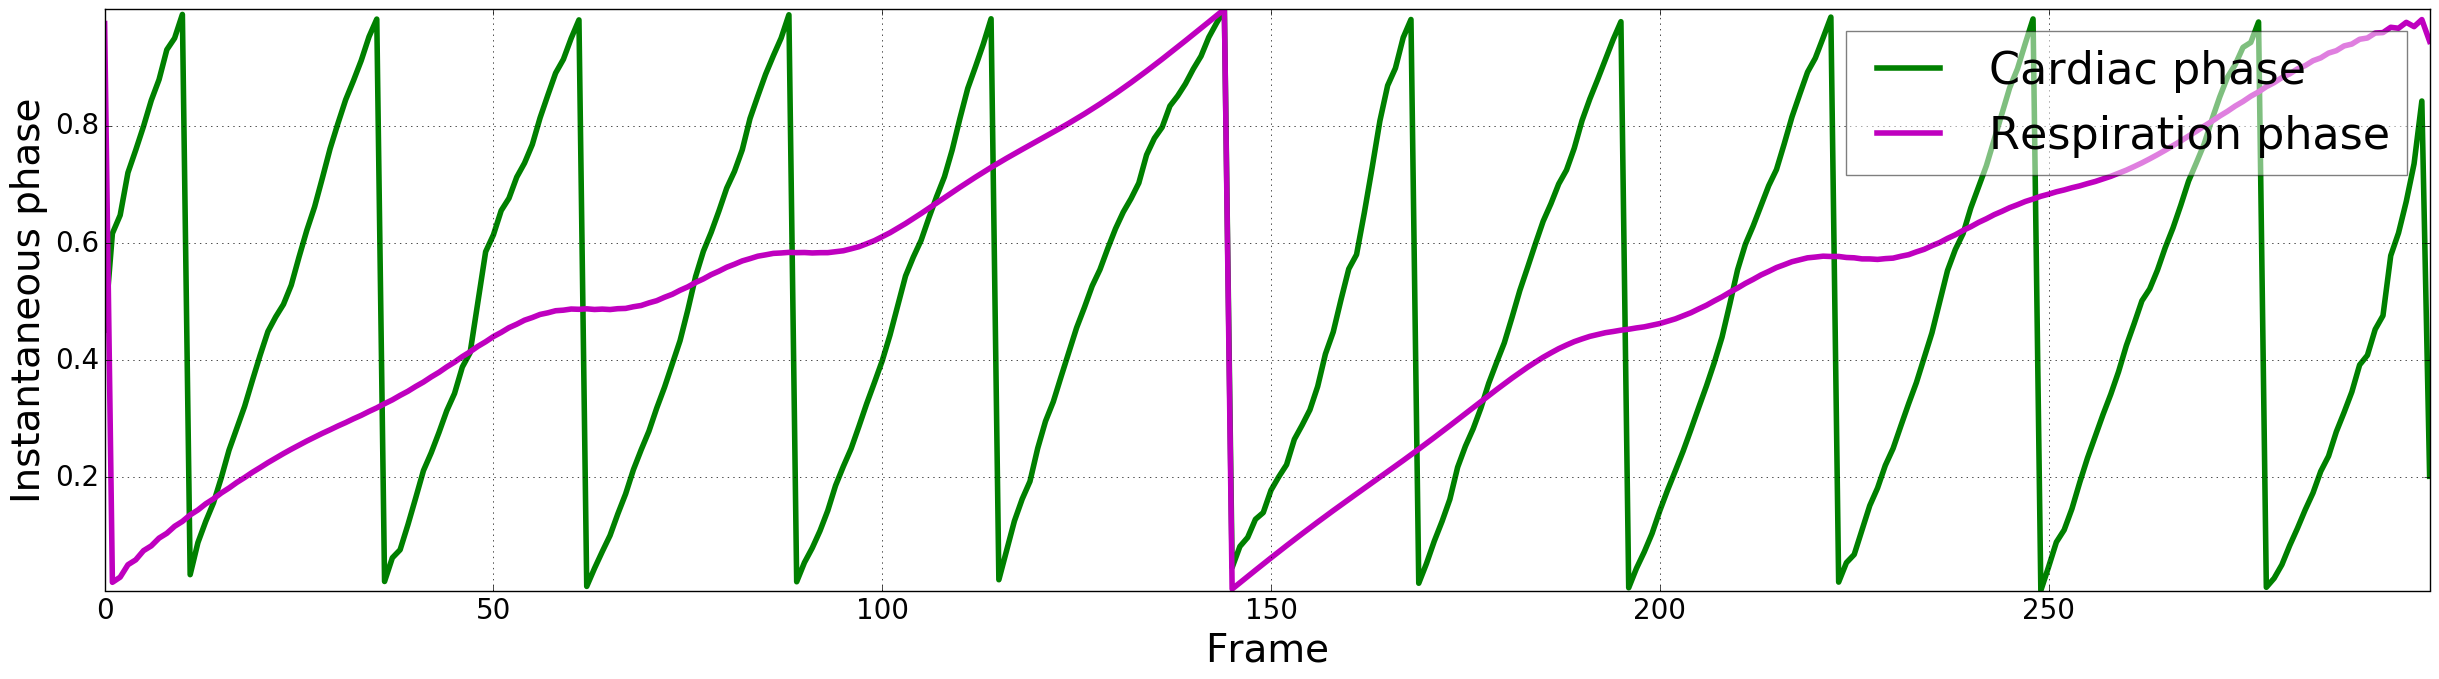
\includegraphics[width=4.75in]{figures/decoded/2015-07-27-10-36-06_2015-07-15-16-56-16_1.raw.bmode/instantaneous_phase.png}
\ionbox{4.75in}\\
%
\caption{Illustration of the proposed phase estimation method: (a) Inter-frame similarity matrix, (b) Trend component corresponding to the respiratory motion, (c) Seasonal component corresponding to the beating heart motion, (d) The similarity profile chosen for phase estimation along with the associated trend/respiration and seasonal/heart-beat components, (e) Periodogram of the heart-beat and respiration components along with the periodicity characteristics such as frequency and cycle duration, and (f) Instantaneous phase of the heart-beat and respiration components.}
\label{fig:phase_estimation}
\end{IonFigT}
%
While there have been numerous efforts for the estimation of instantaneous phase and/or frequency in periodic univariate time series data (wherein a single-variable is measured at each time point)\cite{Boashash1992,Lu2013,Luo2003}, there are not many methods that tackle this problem in a multivariate setting which is the case with periodic cardiac ultrasound videos wherein several thousands of variables (intensities of pixels) could be measured at each time point. Our strategy was to find a way to simplify this seemingly complex multi-variate problem by transforming it into a univariate one and take advantage of existing univariate methods to solve the problem at hand. 

	We first compute the similarity between all pairs of frames in the given periodic image sequence containing $N$ images/frames to create a matrix $A \in R^{N \times N}$ where in the element $A(i,j)$ is equal to the similarity between the $i^{th}$ and $j^{th}$ frames of the given sequence. Here in, we use normalization correlation also known as the Pearson correlation coefficient to quantify inter-frame similarity but, in principle, any of the similarity metrics used in image registration algorithms \cite{Goshtasby2012} can potentially be chosen. Each row in the inter-frame similarity matrix $A$ can now be seen as a univariate time series that measures the similarity of the corresponding frame in the image sequence with all other frames.
If the similarity metric is chosen with care and if the corresponding frame is not significantly corrupted we can expect this time series to encompass the
predominant periodicity characteristics of the original image sequence. Two kinds of periodic motion are present in cardiac ultrasound videos, one corresponding to the beating heart motion and the other corresponding to respiratory motion. Figure \ref{fig:phase_estimation}(a) shows the inter-frame similarity matrix of one of our cardiac ultrasound videos computed using the normalized correlation metric wherein these two sources of periodicity can be clearly observed in the frame similarity signal of many rows/columns. 

	Next, we use a trend extraction technique~\cite{Alexandrov2012} called the Hodrick-Prescott (HP) filter~\cite{Hodrick1997} to decompose the frame similarity signal $u(t)$ into a sum of two components: (i) Trend component $\tau(t)$ encompassing the periodicity characteristic of only the lower-frequency respiratory motion, and (ii) Residual component $r(t)$ encompassing the periodicity characteristic of only the higher-frequency beating heart motion. The HP filter, that is widely used in the field of econometrics, performs the decomposition of $u(t) = \tau(t) + r(t)$ by solving the following optimization problem:
\begin{equation}	
\argmin{\tau(t)} \left[ \sum_{t=1}^{N}  \left(u(t) - \tau(t) \right)^2  + \lambda \sum_{t=1}^{N-1} \left( \nabla^2 \tau(t) \right)^2 \right] 
\end{equation}
where $\nabla^2\tau(t) = \tau(t+1) - 2 \tau(t) + \tau(t-1)$ is the second-order difference or derivative that penalizes curvature of the trend signal. We use a ridge-regression implementation of the Hodrick-prescott filter~\cite{Yamada2015} with $\lambda=6400$. Let $A_r$ and $A_h$ be the matrices whose rows contain the trend/respiratory and the residual/heart-beat components, respectively, of the frame similarity signals in the corresponding rows of the similarity matrix $A$. Figures~\ref{fig:phase_estimation}(b,c) show the trend ($A_r$) and residual ($A_h$) matrices for one of our cardiac ultrasound videos. To minimize the effect of any noise on phase estimation, we pick frame similarity signal corresponding to the row of $A_h$ whose periodogram or power-frequency distribution has minimum entropy. Figure~\ref{fig:phase_estimation}(d) shows the selected frame similarity signal (blue) along with the associated trend/respiration (pink) and residual/heart-beat (green) components. Figure~\ref{fig:phase_estimation}(e) shows the periodogram of these two components. Through Figures~\ref{fig:phase_estimation}(b-e), notice how well the two periodic sources have been decoupled from the raw frame similarity signal. Also, in Figure~\ref{fig:phase_estimation}, notice that most of the energy in the periodogram or power-frequency distribution of the respiration and heart-beat components is concentrated within a narrow frequency band. Furthermore, notice how these 1D signals capture the periodicity characteristics (e.g. frequency in beats-per-minute (bpm), period or cycle duration in frames, number of cycles) of the respective sources of motion in the input high-dimensional periodic image sequence.  
		
	Next, considering the narrow-band nature of the derived trend/respiratory and residual/heart-beat signals, we can use the Hilbert transform~\cite{Lu2013} to estimate the instantaneous intra-period phase of each frame. Specifically, we compute the instantaneous phase $\phi(t) \in \left [  -\pi, \pi\right )$ of the time series $u(t)$ as follows:
\begin{equation}
\phi(t) = arctan \left( \frac{H_u(t)}{u(t)}\right)
\end{equation} 
where $H_u(t)$ is the Hilbert transform of $u(t)$. We map $\phi(t)$ from range $\left [  -\pi, \pi\right )$ to $\left [  0, 1\right )$. Let $\phi_c(t)$ and $\phi_r(t)$ denote the instantaneous heart-beat/cardiac and respiratory phases computed from the trend/respiration and residual/heart-beat signals, respectively, using the aforementioned approach. Figure~\ref{fig:phase_estimation}(f) shows the instantaneous cardiac and respiratory phases computed from the heart-beat and respiration signals in in Figure~\ref{fig:phase_estimation}(d). 

%\vspace{-0.5cm}
\subsection{Gating out respiratory frames}
\label{sec:method:gating}
%
Once the instantaneous cardiac and respiratory phases of each frame has been estimated, it can be used to facilitate the extraction of quantitative measurements from any desired part/point of the periodic cycle, a process commonly referred to as gating. In this section, we present a robust method that uses these phase estimates to gate out video frames predominantly influenced by respiratory motion.

	Firstly, based on the observation that the predominant influence of respiratory motion occurs around the troughs of the trend/respiration component (pink curve in Fig.~\ref{fig:phase_estimation}(d)), we identify the corresponding respiratory phase (equal to phase zero) and perform a rough initial gating by discarding the frames whose respiratory phase distance from it is below a specified cutoff value (we use 0.2). Figure~\ref{fig:respiratory_gating}(a) shows the discarded frames (blue circles) overlaid on the trend/respiration component, residual/heart-beat component, and instantaneous respiratory phase signals.
	
	
	
%
\begin{IonFigT}
\centering
%
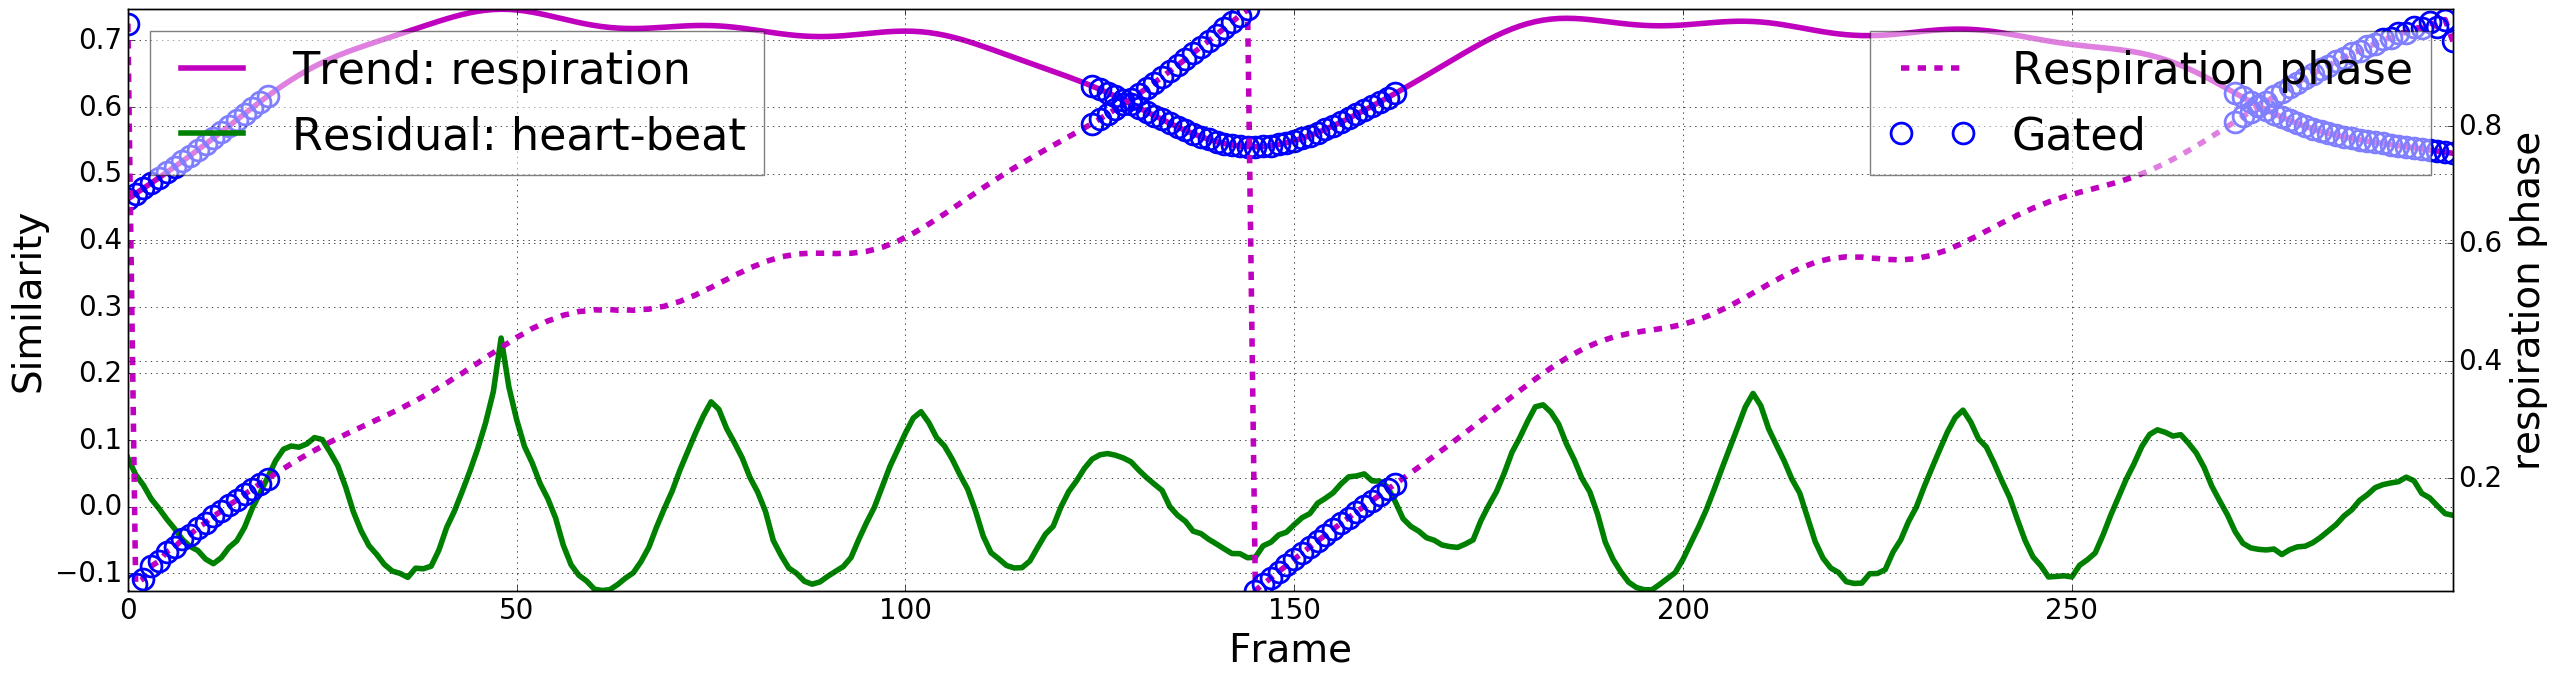
\includegraphics[width=5.0in]{figures/decoded/2015-07-27-10-36-06_2015-07-15-16-56-16_1.raw.bmode/respiratory_phase_gating.png}
\ionbox{5.0in}\\
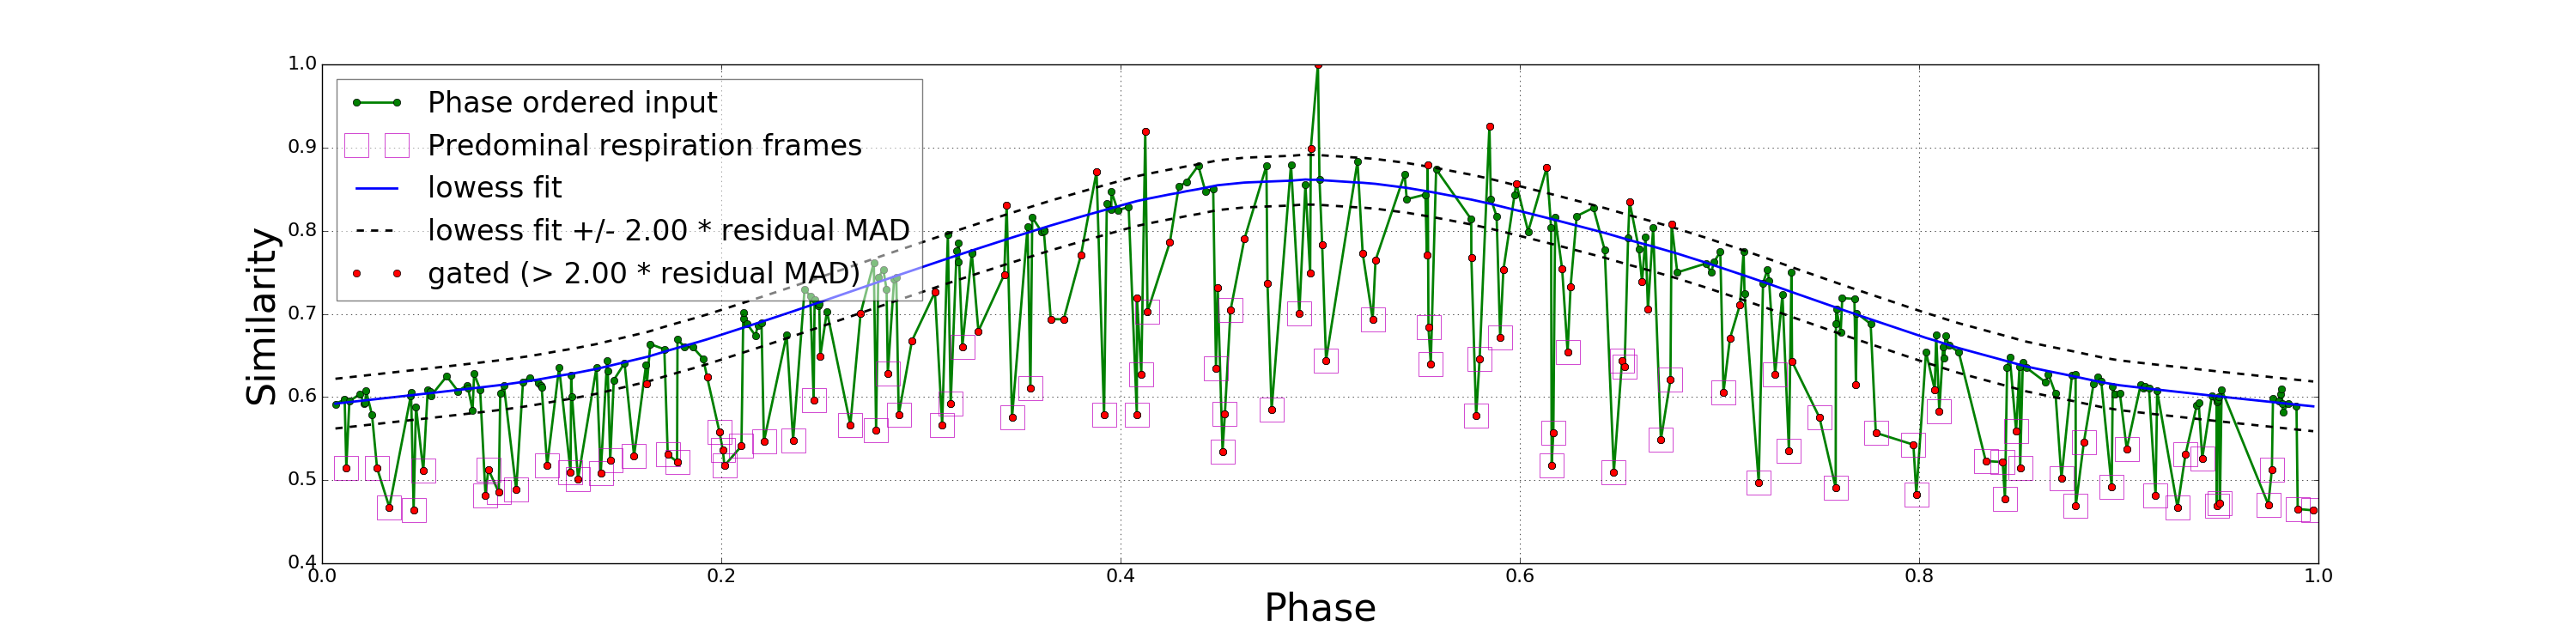
\includegraphics[width=5.0in]{figures/decoded/2015-07-27-10-36-06_2015-07-15-16-56-16_1.raw.bmode/robust_lowess_gating.png}
\ionbox{5.0in}\\
%
\caption{Illustration of our method for gating out respiratory frames: (a) (b)}
\label{fig:respiratory_gating}
\end{IonFigT}
%
%\vspace{-0.5cm}
\subsection{Build model to generate image at any phase for super-resolution}
\label{sec:method:super_resolution}
%
Once the instantaneous cardiac phase of each frame has been estimated, it can be used to enable spatio-temporal super-resolution by considering the set of images within each period of a periodic image sequence as distinct observations of the same data. In this section, we present a method that uses a phase-tagged periodic image sequence to reconstruct a single-period video at a higher temporal resolution. 
	
Given a de-noised periodic sequence $\{L_1, ..., L_n\}$ of $n$ images (with $m$ pixels each) along with their estimated intra-period phases $\{\phi_1, ..., \phi_n\}$, we first use Nadarya-Watson kernel regression\cite{Bishop2006} to construct a phase-parameterized image manifold in the form of a function $M(\phi): [0, 1) \to R^m $ that maps any intra-period phase $\phi$ to an image as follows:
\begin{equation}
M(\phi) = \frac{\sum_{i = 1}^{n} K(\phi, \phi_i) L_i}{\sum_{i = 1}^{n} K(\phi, \phi_i)} 
\end{equation}
where in we define the kernel $K$ using a gausssian with standard-deviation $\sigma$ equal to a multiple of the average distance between consecutive phases after sorting them. Note that, we account for the periodic nature of the intra-period phase whenever we measure distance between two phase values. A single-period video can now be reconstructed by sampling the manifold $M(\phi)$ at any desired resolution from the range $[0, 1)$ of intra-period phase. Note that the aformentioned process will facilitate temporal super-resolution only if the set of images observed in each distinct period of the given image sequence differ in intra-period phase by some non-zero amount less than its temporal sampling interval. Also, the amount of temporal super-resolution possible will depend both on the number of periods observed and the maximum amount by which one can expect the images to be perturbed in phase across observations. 
%\vspace{-0.5cm}
\section{Results}
\label{sec:results}
%
%
\begin{IonFigT}
\centering
%
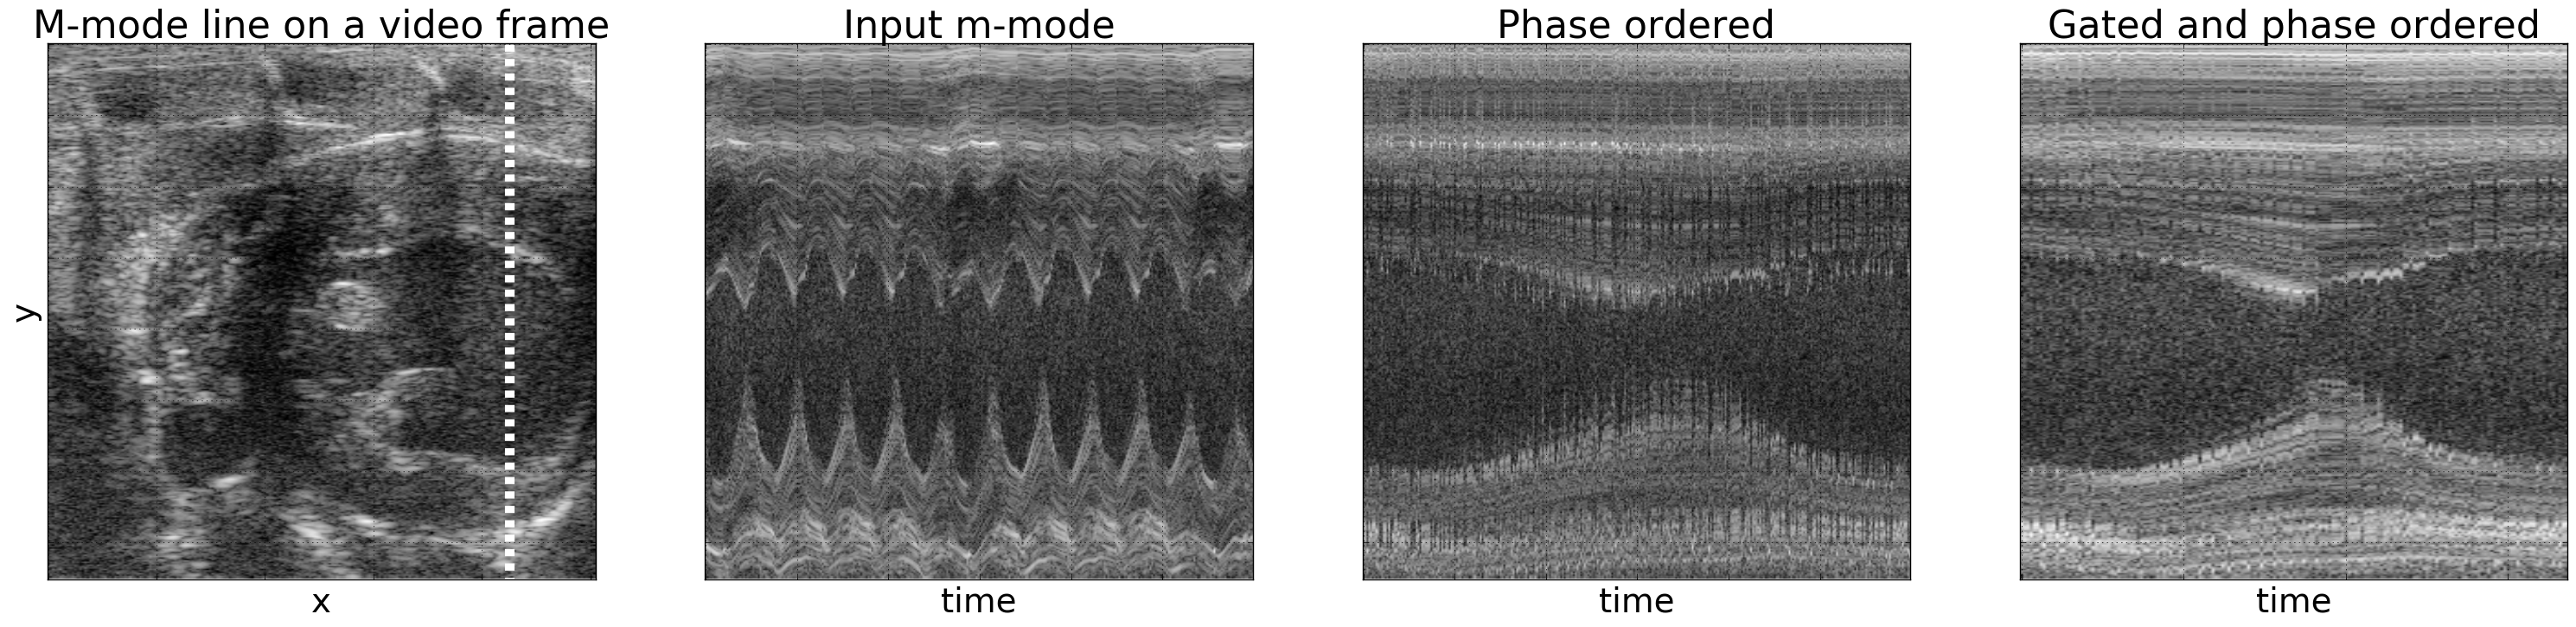
\includegraphics[width=5.0in]{figures/decoded/2015-07-27-10-36-06_2015-07-15-16-56-16_1.raw.bmode/phaseordered.png}
\ionbox{5.0in}\\
%
\caption{Visualization of m-mode frames ordered by estimated cardiac phase}
\label{fig:phase_ordering}
\end{IonFigT}
%
%
%\vspace{-0.5cm}
\section{Discussion and future work}
\label{sec:discussion}
%


%
%\vspace{-0.5cm}
\bibliographystyle{splncs03}
\bibliography{library}
\end{document}







